\documentclass[border=4pt]{standalone}
% Preámbulo común de las figuras. Cada figura es un documento standalone
% que se compila a SVG con scripts/build_figures.sh
\usepackage[utf8]{inputenc}
\usepackage{amsmath}
\usepackage{tikz}
\usepackage[american, siunitx]{circuitikz}
\usetikzlibrary{arrows.meta,calc,decorations.pathmorphing,patterns}
\tikzset{
  >={Stealth[length=2.2mm]},
  eje/.style={->, thin},
  hilo/.style={thick},
}
% Paleta común: tonos medios legibles sobre fondo claro
\definecolor{azul}{RGB}{31,94,168}
\definecolor{rojo}{RGB}{192,57,43}
\definecolor{verde}{RGB}{39,128,73}
\definecolor{naranja}{RGB}{211,120,30}
\definecolor{morado}{RGB}{125,60,152}

\begin{document}
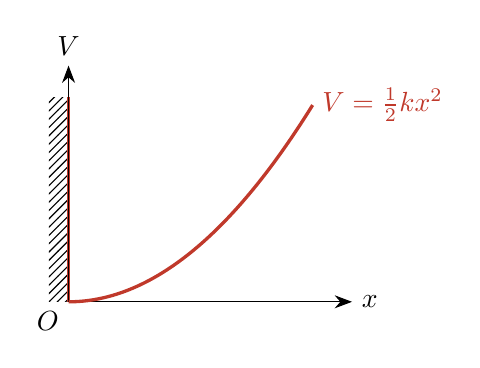
\begin{tikzpicture}[scale=1.0]
  \fill[pattern=north east lines] (-0.25,0) rectangle (0,2.6);
  \draw[very thick, rojo] (0,2.6) -- (0,0);
  \draw[eje] (0,0) -- (3.6,0) node[right]{$x$};
  \draw[eje] (0,0) -- (0,3.0) node[above]{$V$};
  \node[below left] at (0,0) {$O$};
  \draw[very thick, rojo] plot[domain=0:3.1, samples=50] (\x, {0.26*\x*\x});
  \node[right, rojo] at (3.1,2.5) {$V = \tfrac12 kx^2$};
\end{tikzpicture}
\end{document}
